\documentclass[11pt]{article}
\usepackage[margin=1in]{geometry}
\usepackage{amsmath,amssymb,amsthm}
\usepackage{graphicx}
\usepackage{float}
\usepackage{xcolor}
\usepackage{booktabs}
\usepackage{microtype}
\usepackage[numbers,sort&compress]{natbib}
\usepackage{xurl}
\usepackage[colorlinks=true,linkcolor=blue!50!black,citecolor=blue!50!black,urlcolor=blue!50!black]{hyperref}

\emergencystretch=2em
\widowpenalty=10000 \clubpenalty=10000
\makeatletter % a list never starts a page apart from its lead-in
\let\kept@itemize\itemize \def\itemize{\@beginparpenalty\@M\kept@itemize}
\let\kept@enumerate\enumerate \def\enumerate{\@beginparpenalty\@M\kept@enumerate}
\makeatother

\newcommand{\dd}{\mathrm{d}}
\newcommand{\pst}{p_{*h}}
\newcommand{\AH}{{\rm AH}}
% A result that a running task will supply; visible in the PDF until it is replaced.
\newcommand{\pending}[2]{\par\smallskip\noindent\fcolorbox{orange!70!black}{orange!6}{\parbox{\dimexpr\linewidth-2\fboxsep-2\fboxrule}{%
\small\textbf{Pending, #1.} #2}}\par\smallskip}

\title{Near-critical evolution of the Ellis wormhole:\\the type~I lifetime law, the settled black-hole mass\\and the
expanding throat}
\author{Nathan Moinvaziri\thanks{\href{mailto:nathan@nathanm.com}{nathan@nathanm.com}}\\[2pt]
\normalsize\textit{Independent researcher}}
\date{November 2026}

\begin{document}
\maketitle

\begin{abstract}
A static wormhole held open by a massless ghost scalar, the Ellis--Bronnikov wormhole, has one unstable radial mode.
Perturbed, its throat either collapses to a black hole or expands, and between the two outcomes lies a threshold whose
critical solution is the static wormhole itself. We bisect to that threshold in a second-order double-null evolution that
covers both universes, in $D=4$, $5$ and $6$ spacetime dimensions. For pulse families whose threshold data are the
static wormhole, the time spent near it is $(1/W)\ln(1/|p-p_*|)$ plus a constant, with $W$ the growth rate of the
linear mode: over $10^{-9}\le|p-p_*|\le10^{-4}$ two independent codes give the slope $1/W$ to within a relative
$7\times10^{-6}$, $3\times10^{-5}$ and $5\times10^{-4}$ in $D=4$, $5$ and $6$. A one-sided family with an added
normal pulse stalls near an asymmetric static wormhole; read along the throat in its proper time, its slope in $D=4$ is
$0.8495a$, the e-folding time $0.847a$ of that member. In $D=4$ the black hole formed just below threshold settles at
$0.2231a$ (apparent-horizon radius $0.4462a$, $a$ the throat radius) for the symmetric family, the value of
Gonz\'alez, Guzm\'an and Sarbach, and at $0.2355a$ for the one-sided family, where it also depends on the distance from
threshold. Above threshold the symmetric throat's expansion rate grows as $H=k/(\tau_s-\tau)$ in its proper time $\tau$,
with $k=2.0000$ in $D=4$ and $3.99$ in $D=5$: the throat does not approach a de Sitter rate.
\end{abstract}

\tableofcontents

\section{Introduction}\label{sec:intro}

Take the Ellis wormhole of throat radius $a$ in four dimensions and send in a Gaussian pulse of its own ghost field,
with amplitude $p$. Below a threshold amplitude $p_*$ the throat collapses to a black hole; above it the throat expands.
Close to $p_*$ the throat first stalls near its static shape, and the stall lasts longer the closer $p$ is to $p_*$.
Each factor of ten closer buys $1.95a$ of proper time at the throat, because the one unstable mode of the static
wormhole grows by a factor $e$ every $0.846a$. This paper measures that law, the mass of the black hole that forms, and
what the throat does when it expands.

The wormhole is the static, spherically symmetric solution of Einstein gravity with a massless scalar whose kinetic
term has the wrong sign (a ghost), found by Ellis and by Bronnikov~\cite{Ellis1973,Bronnikov1973}. Gonz\'alez,
Guzm\'an and Sarbach showed that its spherical perturbations have exactly one growing mode, for the symmetric member and
for the asymmetric members whose two asymptotic masses differ~\cite{GGS2009a}, and Torii and Shinkai found one growing
mode in every dimension they computed~\cite{TS2013}. Its growth rate $W$ is known to many digits in $D=4$--$2000$ and in
closed form at large $D$~\cite{P3}.

Shinkai and Hayward evolved the four-dimensional wormhole in double-null coordinates through both universes and found
the two fates, collapse and expansion, separated by a sharp boundary that they called ``a new kind of critical behaviour
reminiscent of that found by Choptuik''~\cite{SH2002}. Near it they saw a black-hole mass tending to $0.30a$, a
formation time growing as $0.60\ln(1/E_0)$ in their null coordinate, with $E_0$ the injected energy, and an expanding
throat with a fitted rate $1.1/a$. Gonz\'alez, Guzm\'an and Sarbach repeated the evolutions in Cauchy form and found a
final apparent-horizon radius $0.45a$ as the perturbation vanishes, an expanding branch whose e-folding time tends to
$0.85a$, and a second collapse window on the expanding side~\cite{GGS2009b}. Shinkai and Torii extended the runs to
$D=5$ and $6$ and to Einstein--Gauss--Bonnet gravity, and found a final mass that does not depend on the injected
energy~\cite{ST2017}. Recent evolutions show the same two fates in double-null~\cite{XCY2025} and in other
codes~\cite{Kain2026}, and a $3+1$ study of a massive Ellis--Bronnikov throat describes the static throat as
``consistent with a type-I critical solution'' while its two amplitudes ``do not establish the scaling''~\cite{SN2026}.

These are the signatures of type~I critical collapse~\cite{CCB1996,GMG2007,GHMG2025}: a static critical solution with
one unstable mode, a lifetime $T\simeq(1/W)\ln(1/|p-p_*|)$ and a finite black-hole mass at threshold. Our companion paper~\cite{P3}
converted Shinkai and Hayward's exponent to proper time and found $0.60\sqrt2\,a=0.85a$ against $1/W=0.846a$, and
compared two-run slopes of Shinkai and Torii with $1/W$ in $D=5$ and $6$.
% NOVELTY: check literature.md
None of the runs above bisects to the threshold: \cite{SH2002} fits two decades of $E_0$, \cite{ST2017} gives two
amplitudes per dimension, and \cite{SN2026} two amplitudes. The two published threshold masses, $0.30a$~\cite{SH2002}
and $0.22a$~\cite{GGS2009b}, disagree, and the expanding branch has been read as inflationary~\cite{SH2002} or as an
exponential expansion~\cite{GGS2009b} from runs that stop a few e-folds after the departure.

This paper gives the full account of a bisection study in a double-null code that passes the throat. Reference~\cite{P3}
summarizes part of it in its threshold section. The contributions are:
\begin{itemize}
\item \emph{The threshold is resolved by bisection.} The discrete threshold $\pst$ converges at second order in the grid
spacing $h$, and for families through the static wormhole $\pst\propto h^2$: truncation error alone seeds the unstable
mode (Sec.~\ref{sec:pstar}).
\item \emph{The lifetime law holds with the slope $1/W$} in $D=4$, $5$, $6$ over five to eight decades of
$|p-\pst|$, confirmed by a second code that shares only the field equations (Sec.~\ref{sec:life}).
\item \emph{A one-sided family approaches an asymmetric static member.} Read along the throat's locus, its slope is that
member's e-folding time in $D=4$; in $D=5$ the member's radius drifts during the stall (Sec.~\ref{sec:locus}).
\item \emph{The settled black-hole mass} is $0.2231a$ for the symmetric family, $0.0125a$ less than for the one-sided
family, whose value also depends on the distance from threshold; Shinkai and Hayward's $0.30a$ is not reproduced with
their own data (Sec.~\ref{sec:mass}).
\item \emph{The expanding throat} has $1/H$ linear in its proper time, so its areal radius and curvature diverge at a
finite proper time on the extrapolated fit; its isotropic equation of state is fixed by symmetry
(Sec.~\ref{sec:expand}).
\end{itemize}
Section~\ref{sec:limits} lists what follows and what is open, and Sec.~\ref{sec:computations} what was checked and how.
Every number below is \emph{numerical evidence} unless it is marked otherwise.

\section{Setting}\label{sec:setting}

\subsection{The Ellis wormhole in \texorpdfstring{$D$}{D} dimensions}

Let $D=n+2$ and use units with $8\pi G=1$. Einstein gravity with massless scalars $\phi_k$ of sign $\varepsilon_k$
($+1$ normal, $-1$ ghost) has $R_{ab}=\sum_k\varepsilon_k\,\partial_a\phi_k\partial_b\phi_k$ and $\Box\phi_k=0$. The
symmetric Ellis wormhole of throat radius $a$ is
\begin{equation}
\dd s^2=-\dd t^2+\dd l^2+r(l)^2\dd\Omega_n^2,\qquad r'^2=1-(a/r)^{2(n-1)},\qquad \phi'=q/r^n,\qquad q^2=n(n-1)a^{2n-2},
\label{eq:ellis}
\end{equation}
with the ghost sign; in $D=4$, $r=\sqrt{l^2+a^2}$~\cite{Ellis1973,Bronnikov1973}, and Torii and Shinkai give the
$D$-dimensional form~\cite{TS2013}. The proper distance $l$ runs from one universe ($l<0$) to the other ($l>0$), and
both ends are asymptotically flat with zero mass. Its single unstable radial mode grows as $e^{Wt}$ in the proper time
$t$ at the throat~\cite{GGS2009a,TS2013}. We take $W$ from the quad-double integration of Ref.~\cite{P3}:
$W^2a^2=1.39705243433350684$, $2.98495893035176025$ and $4.68662054311946479$ in $D=4$, $5$ and $6$, so the e-folding
time is $1/(Wa)=0.846045$, $0.578803$ and $0.461924$. The static family has a second parameter, the asymmetry $\gamma_1$
of Ref.~\cite{GGS2009a}: its members have opposite-sign masses at the two ends, and in $D=4$ their e-folding time is
$T(\gamma_1)\,r_{\rm th}$, with $r_{\rm th}$ the throat radius and $T$ the function computed in
Ref.~\cite{GGS2009a} ($T(0)=1/(Wa)$).

\subsection{Three families of initial data}\label{sec:families}

Each family adds a Gaussian pulse $\delta\phi=p\,[g(x^+)-g(0)]$, $g(s)=\exp(-(s-3a)^2/(0.5a)^2)$, to the static data on
the null ray $x^-=0$ of Sec.~\ref{sec:scheme}. It is centred at proper distance $l=3a/\sqrt2$ and falls into the throat.
\begin{itemize}
\item \textbf{S} (symmetric): a ghost pulse of amplitude $p$ on the ray $x^-=0$, mirrored with odd parity onto $x^+=0$,
so the data are reflection symmetric.
\item \textbf{O} (one-sided): the same ghost pulse on $x^-=0$ only.
\item \textbf{G} (one-sided, generic): the ghost pulse of amplitude $p$ plus a pulse of a second, normal scalar of fixed
amplitude $B=0.1$, of the same shape on the same ray.
\end{itemize}
The parameter $p$ is tuned; $p_*$ denotes its threshold value and $\pst$ the value found at grid spacing $h$. The
reflection $l\to-l$, $\phi\to-\phi$ maps the static wormhole to itself. The unstable mode is even under it and the
asymmetric zero mode (the move to $\gamma_1\ne0$) is odd. The even part of the O data of amplitude $p$ is the S data of
amplitude $p/2$, so O's threshold is twice S's, and O also excites the zero mode. G is the only family whose threshold
data are not the static wormhole.

\subsection{The double-null scheme}\label{sec:scheme}

The metric is
\begin{equation}
\dd s^2=-2e^{-f}\dd x^+\dd x^-+r^2\dd\Omega_n^2,
\end{equation}
with $r$, $f$ and $\phi_k$ functions of the null coordinates $x^\pm$. The field equations reduce to three wave
equations and two constraints (Appendix~\ref{app:equations}):
\begin{gather}
r_{+-}=-(n-1)\,\frac{r_+r_-+e^{-f}/2}{r},\qquad f_{+-}=\frac{n}{r}\,r_{+-}+\sum_k\varepsilon_k\phi_{k+}\phi_{k-},
\label{eq:evol}\\
\phi_{k+-}=-\frac{n}{2r}\,(r_+\phi_{k-}+r_-\phi_{k+}),\label{eq:evolphi}\\
C_{\pm\pm}\equiv r_{\pm\pm}+f_\pm r_\pm+\frac{r}{n}\sum_k\varepsilon_k\phi_{k\pm}^2=0,\label{eq:constraints}
\end{gather}
where subscripts $\pm$ are derivatives in $x^\pm$. For $n=2$ these are Shinkai and Hayward's equations~\cite{SH2002},
and Shinkai and Torii use the same dual-null form in higher $D$~\cite{ST2017}. The Misner--Sharp mass
\begin{equation}
M=\tfrac12\,r^{n-1}\left(1+2e^{f}r_+r_-\right)\label{eq:ms}
\end{equation}
satisfies $(\nabla r)^2=1-2M/r^{n-1}$~\cite{MisnerSharp1964}; in $D=4$ a marginally trapped sphere has $M=r/2$. A sphere
is trapped where $r_+<0$ and $r_-<0$, and anti-trapped where both are positive.

Data are given on the two null rays $\Sigma^+=\{x^-=0\}$ and $\Sigma^-=\{x^+=0\}$, which meet at the throat sphere S
(Fig.~\ref{fig:domain}). The gauge is $f=0$ on the rays. For the static wormhole $f\equiv0$ and $x^\pm=(t\pm l)/\sqrt2$,
so $t=(x^++x^-)/\sqrt2$ is its proper time at the throat. On each ray the constraint is linear in $r$ once $f$ and the
$\phi_k$ are given, and it is solved by a fourth-order Runge--Kutta step. The evolved region is the square
$[0,X]^2$, the domain of dependence of the data: it has no outer boundary, both universes are in it, and the throat line
$x^+=x^-$ leaves it at $t=\sqrt2X$. A second-order predictor--corrector (diamond) update advances
Eqs.~\eqref{eq:evol}--\eqref{eq:evolphi} on a uniform grid of spacing $h$ in $x^\pm$, the scheme of Refs.~\cite{SH2002,ST2017}. Cells with
$r<0.05a$ or $e^{-f}>25$ are excised with their future. The constraints~\eqref{eq:constraints} are monitored, not
imposed. The square has $X=28$, $18$ and $15$ for S and O in $D=4$, $5$, $6$, and $X=28$, $22$, $28$ for G.

\begin{figure}[tbp]
\centering
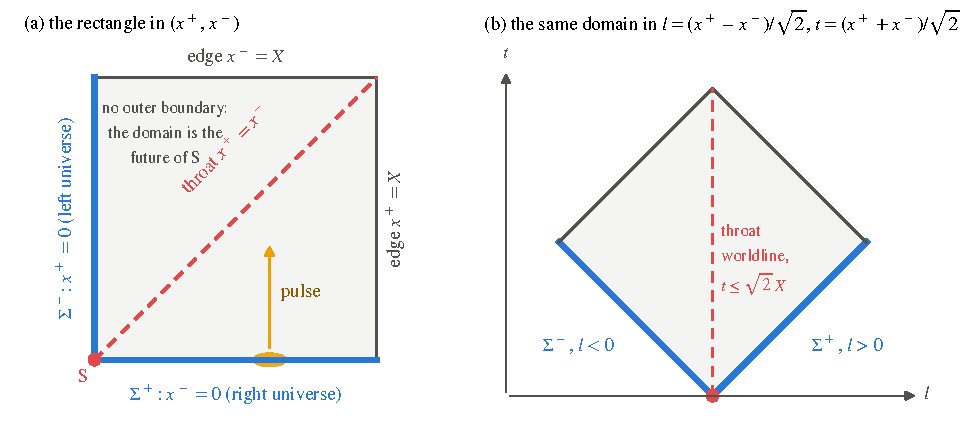
\includegraphics[width=\linewidth]{fig_domain.pdf}
\caption{The domain of the double-null evolution. Data are given on the null rays $\Sigma^\pm$, which meet at the throat
sphere S of the static wormhole. The square $[0,X]^2$ is the future of S inside the data's domain of dependence, so it
has no outer boundary and contains both universes. A pulse on $\Sigma^+$ falls into the throat and reaches it at
$x^-=3a$.}
\label{fig:domain}
\end{figure}

\subsection{Events, lifetimes and fits}\label{sec:events}

The x$^-$ sweep stops at the first event:
\begin{itemize}
\item \emph{collapse}, the first row with a trapped cell, $r_+<-10^{-2}$ and $r_-<-10^{-2}$;
\item \emph{expansion}, the first row whose cell on the line $x^+=x^-$ has $r_\pm>10^{-2}$ and $r\ge2a$.
\end{itemize}
The lifetime $T$ is $t$ at the event cell. For each family the threshold is bisected until the bracket is at most
$10^{-14}$, and then $T$ is measured at $p=\pst\mp10^{-e}$ for $e=3,3.5,\ldots,12$. The fit is
\begin{equation}
T=c_\pm+s\,\ln\frac{1}{|p-\pst|},\label{eq:fit}
\end{equation}
with one slope $s$ and one constant per side. The primary window is $10^{-11}\le|p-\pst|\le10^{-3}$. Three kinds of
error bar are kept apart. The \emph{OLS SE} is the standard error of the primary fit; it assumes independent residuals
(the event row quantizes $T$ by about $h$). The \emph{fit spread} is the envelope of $s\pm2\,$SE over 15 fits, five
windows times (joint, collapse side, expansion side); it measures the dependence on those choices. The \emph{resolution
difference} is the change of the slope between the two finest $h$. The grid spacings are $h=0.02$, $0.01$, $0.005$ in
$D=4$, $0.01/\sqrt2$, $0.005/\sqrt2$, $0.0025/\sqrt2$ in $D=5$, and $0.005$, $0.0025$, $0.00125$ in $D=6$, all in units
of $a$; G in $D=6$ was run at the first two only.

\section{Results}\label{sec:results}

\subsection{The threshold, and \texorpdfstring{$\pst\propto h^2$}{p*h ~ h2}}\label{sec:pstar}

Table~\ref{tab:pstar} gives $\pst$ at the three grid spacings. For S and O, $\pst$ falls by a factor four per halving of
$h$, and the second-order Richardson extrapolation is zero to within $8.1\times10^{-7}$. For G it converges at second
order to $p_*=1.4855\times10^{-2}$ in $D=4$ and $1.0681\times10^{-2}$ in $D=5$. O's threshold is twice S's to a relative
$10^{-3}$ at every $h$, as the decomposition of Sec.~\ref{sec:families} requires.

\begin{table}[tbp]
\centering
\caption{The discrete threshold $\pst$ at the three grid spacings of Sec.~\ref{sec:events} (coarse to fine), the observed
order of convergence from the three values, and the second-order Richardson extrapolation. G in $D=6$ has two spacings,
whose ratio is $1.1416$.}
\label{tab:pstar}
\small
\begin{tabular}{rllllll}
\toprule
$D$ & family & $\pst(h_1)$ & $\pst(h_2)$ & $\pst(h_3)$ & order & Richardson $p_*$ \\
\midrule
4 & S & $4.7528\times10^{-5}$ & $1.1884\times10^{-5}$ & $2.9712\times10^{-6}$ & 2.000 & $-7.4\times10^{-10}$ \\
4 & O & $9.5052\times10^{-5}$ & $2.3768\times10^{-5}$ & $5.9423\times10^{-6}$ & 2.000 & $-1.7\times10^{-9}$ \\
4 & G & $1.4946\times10^{-2}$ & $1.4877\times10^{-2}$ & $1.4860\times10^{-2}$ & 2.000 & $1.4855\times10^{-2}$ \\
5 & S & $2.8848\times10^{-4}$ & $7.2091\times10^{-5}$ & $1.8021\times10^{-5}$ & 2.001 & $9.6\times10^{-9}$ \\
5 & O & $5.7699\times10^{-4}$ & $1.4418\times10^{-4}$ & $3.6042\times10^{-5}$ & 2.001 & $2.1\times10^{-8}$ \\
5 & G & $1.1233\times10^{-2}$ & $1.0819\times10^{-2}$ & $1.0716\times10^{-2}$ & 2.001 & $1.0681\times10^{-2}$ \\
6 & S & $1.1155\times10^{-3}$ & $2.7784\times10^{-4}$ & $6.9396\times10^{-5}$ & 2.007 & $3.5\times10^{-7}$ \\
6 & O & $2.2329\times10^{-3}$ & $5.5579\times10^{-4}$ & $1.3880\times10^{-4}$ & 2.008 & $8.1\times10^{-7}$ \\
6 & G & $1.2658\times10^{-2}$ & $1.1088\times10^{-2}$ & -- & -- & -- \\
\bottomrule
\end{tabular}
\end{table}

\paragraph{Reading.} For S and O the threshold data are the static wormhole itself. The scheme's truncation error, of
order $h^2$, excites the unstable mode at $t=0$, and the bisection finds the pulse amplitude that cancels that seed.
That amplitude is $\pst\propto h^2$, and it vanishes in the continuum. The code therefore holds the static wormhole for
as long as one likes once $p$ is tuned, and the lifetime measures how fast the mode grows away from it. G's threshold
is a finite pulse, and its $\pst$ moves with $h$ only by its truncation error.

The bisection is carried to a bracket of $10^{-14}$, below what $\pst$ means. Below $|p-\pst|\approx10^{-11}$ the
lifetime stops being a smooth function of $p$, and at $|p-\pst|\lesssim10^{-12}$ points land on the wrong side of
$\pst$: roundoff in the evolution, amplified along the unstable mode, decides the fate there. So $\pst$ is determined to
about $10^{-12}$, and the fits stop at $10^{-11}$.

\pending{\#227}{The roundoff floor of $\pst$: an extended-precision bisection, and the roundoff seed of the unstable
mode against the floor near $10^{-11}$. This paragraph will state the measured floor and its cause.}

\subsection{The lifetime law against \texorpdfstring{$1/W$}{1/W}}\label{sec:life}

Figure~\ref{fig:lifetime} shows $T$ against $\ln(1/|p-\pst|)$ for S at the finest $h$, and Table~\ref{tab:life}
collects the slopes. For S and O, $1/W$ lies inside the fit spread at every $D$ at the two finest $h$. Over the primary
window the slope of S at the finest $h$ is within $5.63\times10^{-4}$, $3.88\times10^{-4}$ and $4.97\times10^{-3}$ of
$1/W$ (relative) in $D=4$, $5$, $6$.

A second code, written independently for the review (Sec.~\ref{sec:computations}), evolves S on the half $x^+\ge x^-$ with its own diamond
scheme and its own ray data, places the events where the throat crosses $r=a/2$ or $r=2a$, interpolated in $t$, and
fits over $10^{-9}\le|p-\pst|\le10^{-4}$. Its slope differs from $1/W$ by $-2.55\times10^{-6}$, $-2.48\times10^{-5}$
and $-4.74\times10^{-4}$ (relative) in $D=4$, $5$, $6$ at the finest $h$, and the difference falls with
$h$, by a factor of $2.7$ to $5.4$ per halving. The first code's own points refitted over the same window give
$0.846040$, $0.578786$ and $0.461770$, which differ from $1/W$ by $-6.3\times10^{-6}$, $-2.9\times10^{-5}$ and
$-3.3\times10^{-4}$; the two codes agree to $3.73\times10^{-6}$, $4.33\times10^{-6}$ and $1.41\times10^{-4}$. In the
throat's proper time the second code's slope equals its slope in $t$ to $10^{-5}a$.

The primary window's $D=6$ slope lies $0.5\%$ below the refit. The difference comes from the decade
$10^{-4}<|p-\pst|\le10^{-3}$, where the collapse side is not yet logarithmic.

\begin{figure}[tbp]
\centering
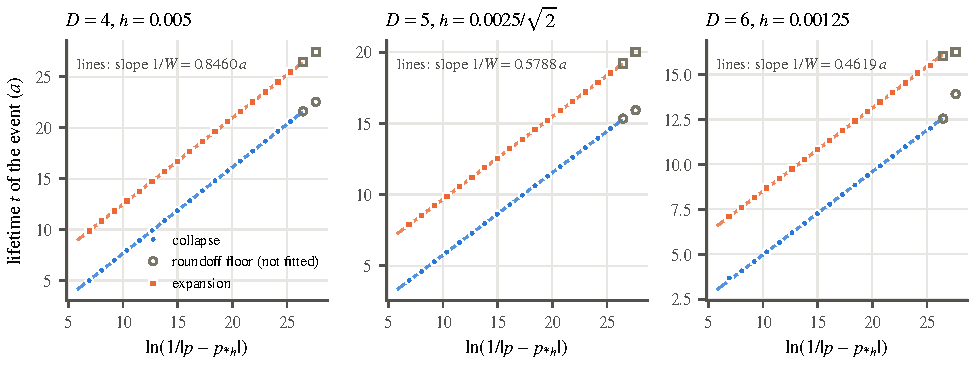
\includegraphics[width=\linewidth]{fig_lifetime.pdf}
\caption{Lifetime $t$ of the event against $\ln(1/|p-\pst|)$ for the symmetric family S at the finest grid spacing.
Filled points ($e\le11$) enter the fit; open gray points lie on the roundoff floor and do not. The lines have slope
$1/W$ and one intercept per side, fixed by the mean offset of that side's points; they are not fitted slopes.}
\label{fig:lifetime}
\end{figure}

\begin{table}[tbp]
\centering
\caption{The lifetime slope $s$ of Eq.~\eqref{eq:fit}, in units of $a$, at the finest grid spacing (G in $D=6$:
$h=0.0025$). First code: events on the grid, primary window $10^{-11}$ to $10^{-3}$, $s\pm$ OLS SE, and the fit spread.
Refit: the same points over $10^{-9}$ to $10^{-4}$. Second code: the reviewer's independent code, same window.
G is read on the line $x^+=x^-$, and in the proper time $\tau$ of the throat's locus (Sec.~\ref{sec:locus}).}
\label{tab:life}
\small
\setlength{\tabcolsep}{4pt}
\begin{tabular}{rllllll}
\toprule
$D$ & $1/(Wa)$ & family & first code, $s\pm$ SE & fit spread & refit & second code \\
\midrule
4 & 0.846045 & S & $0.846522\pm0.000261$ & $[0.845723, 0.848441]$ & 0.846040 & 0.846043 \\
 & & O & $0.845867\pm0.000168$ & $[0.844639, 0.846716]$ & & \\
 & & G, line & $0.899089\pm0.005454$ & $[0.864070, 0.958277]$ & & \\
 & & G, locus $\tau$ & $0.849489\pm0.000231$ & $[0.848180, 0.851639]$ & & \\
\addlinespace
5 & 0.578803 & S & $0.579027\pm0.000229$ & $[0.578002, 0.580219]$ & 0.578786 & 0.578789 \\
 & & O & $0.578966\pm0.000285$ & $[0.577095, 0.581630]$ & & \\
 & & G, line & $0.800277\pm0.015565$ & $[0.709379, 0.938761]$ & & \\
 & & G, locus $\tau$ & $0.702185\pm0.005149$ & $[0.665997, 0.752506]$ & & \\
\addlinespace
6 & 0.461924 & S & $0.459628\pm0.000868$ & $[0.455143, 0.462600]$ & 0.461770 & 0.461705 \\
 & & O & $0.460325\pm0.000791$ & $[0.452896, 0.465270]$ & & \\
 & & G, line & $0.994756\pm0.026714$ & $[0.798040, 1.200660]$ & & \\
\bottomrule
\end{tabular}
\end{table}

The slopes are also stable in $h$: between the two finest spacings the primary slope of S changes by
$2.76\times10^{-5}$ in $D=5$ and $1.35\times10^{-3}$ in $D=6$, within the bar of $0.5\%$ set before the runs. In $D=4$
the two finest slopes coincide, because the event rows of the two spacings agree to within one coarse row.

\paragraph{Reading.} Data tuned to the static wormhole leave it at the rate of its linear mode, in a fully nonlinear
evolution, and the lifetime law holds to the precision the event definition allows. The large-$D$ expansion of Ref.~\cite{P3}
then gives $T\simeq a\ln(1/|p-p_*|)/\sqrt{2(D-3)}$ at large $D$. This is a test of the growth rate along the
static solution's unstable direction, not of how generic data approach it: in S and O the data start on the static
wormhole, perturbed by $p$ and by the truncation error. The earlier measurements fit the same law. Shinkai and Hayward's
exponents $0.60$ (ghost pulses) and $0.61$ (normal pulses) in $x^-$, against the predicted $1/(\sqrt2W)=0.598$, and
two-run slopes from Shinkai and Torii's table, $0.71\pm0.14$, $0.43\pm0.02$ and $0.335\pm0.011$ against $0.598$,
$0.409$ and $0.327$ in $D=4$, $5$, $6$, are compared in Ref.~\cite{P3}.

\subsection{The one-sided family on the throat's locus}\label{sec:locus}

Read on the line $x^+=x^-$, as for S, family G gives slopes above $1/W$ by $6\%$, $38\%$ and $115\%$ in $D=4$, $5$, $6$,
the same at each $h$ (Table~\ref{tab:life}). That line is not the throat for G. Define the \emph{locus} as the minimum of
$r$ on each slice $t=$ const, with position $l(t)$, drift $v=\dd l/\dd t$ and proper time
$\dd\tau=e^{-f/2}\sqrt{1-v^2}\,\dd t$; the lifetime is $\tau$ where $r$ on the locus reaches $a/2$ (collapse) or $2a$
(expansion). The same runs, read on the locus, give the slopes of Table~\ref{tab:life} and Fig.~\ref{fig:locus}.

In $D=4$ the locus slope is $0.849542$, $0.849536$ and $0.849489$ at the three $h$, the two finest agreeing to
$5.52\times10^{-5}$, while the line slope of the same runs is reproduced to the last digit. Reading $t$ instead of $\tau$
on the locus gives $0.870859$: the lapse at the locus accounts for part of the excess, the drift for the rest. A
planted test separates the observer from the physics: family S in coordinates rescaled so that the static throat drifts
at $v=0.1$ reads $0.846052$ on the locus ($+8.44\times10^{-6}$ against $1/W$) and $0.912185$ on the line ($+7.82\%$).

The state at the stall is a static member. Fitting the Misner--Sharp mass on the two sides of the locus, at
$r=1.25$ to $4$ times the throat radius, to the asymmetric static family gives at $t=12a$ the throat radius
$r_{\rm th}=1.0031a$ and asymmetry $\gamma_1=0.048$, and $r_{\rm th}=1.0028a$ at $t=13a$ and $14a$; the throat radius changes
by $-0.0023a$ from $t=10a$ to $15a$. The second field carries no charge there: its share of the static charge is
below $10^{-5}$. The member's e-folding time $T(\gamma_1)\,r_{\rm th}$~\cite{GGS2009a} is $0.8474a$, and the growth
rate of the unstable mode measured from two runs at $\pst\mp10^{-9}$ gives $0.8478a$. The series slope $0.8495a$ is
within $0.25\%$ of both.

In $D=5$ there is no plateau. The locus radius grows from $1.0715a$ to $1.1974a$ between $t=7a$ and $13a$, and the
mode's measured rate follows $W/r_{\rm th}(t)$, the symmetric member's rate at the current radius, to within $0.51\%$
along the way. The series slope, $0.702185a$ at the finest $h$, is then an average over a drifting member, and the
local slope rises with $\ln(1/|p-\pst|)$ (Fig.~\ref{fig:locus}).

\begin{figure}[tbp]
\centering
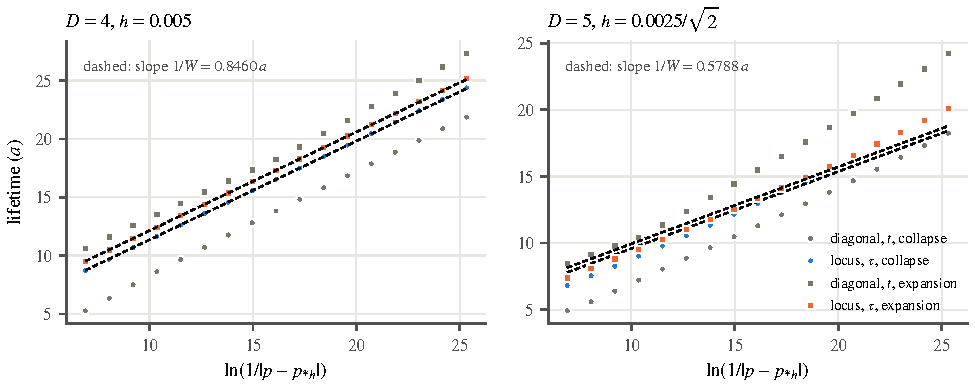
\includegraphics[width=\linewidth]{fig_locus.pdf}
\caption{Family G at the finest grid spacing. Gray: lifetime $t$ on the line $x^+=x^-$ with the events of
Sec.~\ref{sec:events}. Colored: proper time $\tau$ of the throat's locus where its radius reaches $a/2$ or $2a$. Dashed:
slope $1/W$ through the locus points. In $D=4$ the locus points follow a straight line of slope $0.8495a$; in $D=5$ the
slope rises with $\ln(1/|p-\pst|)$ as the stall member's radius drifts.}
\label{fig:locus}
\end{figure}

\paragraph{Reading.} In $D=4$ the one-sided family is critical in the same sense as S: it stalls near one static
wormhole and leaves it at that wormhole's rate. The wormhole is not the symmetric one but a slightly asymmetric member,
and the excess of $6\%$ on the line is the observer's, not the critical solution's. In $D=5$ the stall does not settle
onto one member, so the lifetime is not a single logarithm over the range measured.

\pending{\#255}{What drives the drift of the stall member's radius in $D=5$, and whether G's expanding member in $D=5$
follows Eq.~\eqref{eq:ft} on a longer run. This subsection will add both.}

\subsection{The settled black-hole mass}\label{sec:mass}

In S and O the Misner--Sharp mass at the first trapped cell is $0.494$, $0.492$ and $0.490a^{D-3}$ in $D=4$, $5$, $6$,
at $r\approx0.99a$: the horizon forms at the stalled throat. It is not the final mass. After formation $e^{-f}$ grows exponentially along the
apparent horizon (the outermost sphere with $r_+=0$), so on a uniform grid the horizon becomes a layer narrower than a
cell. We follow it with a chain of grids. Each level halves the step in $x^-$ and starts at the column where $e^{-f}$ on
the horizon reaches $1.5\times2^k$, with its lower ray a row of the previous level and its left ray that level's column,
interpolated by cubic splines. Characteristic evolution has no dependence on later $x^\pm$, so each level is exact in
its domain of dependence. Twenty levels reach $e^{-f}=1572864$ on the horizon. The horizon is the zero of $r_+$ in each
column and $M_\AH=r_\AH/2$ there (in $D=4$).

Figure~\ref{fig:mass} and Table~\ref{tab:mass} give $M_\AH$ for S and G in $D=4$ at $p=\pst-\delta$. For S it falls
from $0.49424a$ at the first trapped cell, is $0.30315a$ at $x^+-x^+_f=2.5a$, and settles at $0.223083a$
($r_\AH=0.44617a$) at $h=0.0025$, with $x^+_f$ the formation point. The two finest $h$ differ by $2.13\times10^{-6}$, the
plateau over its last unit of $x^+$ ranges over $2.6\times10^{-6}$, and $\delta=10^{-6}$ and $10^{-8}$ differ by
$7.0\times10^{-8}$. The same code on another machine reproduced the value at $h=0.01$ to $1.6\times10^{-5}$, so we
quote
$M_\AH=0.2231a$ ($r_\AH=0.4462a$). It is the same, $0.2231a$, for every $\delta$ from $10^{-8}$ to $10^{-3}$.

\begin{table}[tbp]
\centering
\caption{Mass on the apparent horizon in $D=4$, in units of $a$, at $h=0.005$ unless stated. ``Settled'' is the mean
over the last unit of $x^+$, ending at $e^{-f}=1.57\times10^6$ on the horizon. The rows below the line are different
kinds of error bar and are not to be added: a resolution difference, an extrapolation and a physical dependence.}
\label{tab:mass}
\small
\begin{tabular}{lll}
\toprule
& S & G \\
\midrule
at the first trapped cell, $\delta=10^{-8}$ & 0.49421 & 0.49550 \\
settled, $\delta=10^{-8}$ & 0.223085 & 0.235548 \\
apparent-horizon radius $r_\AH$ & 0.4462 & 0.4711 \\
\midrule
$|M(h=0.01)-M(h=0.005)|$ & $1.63\times10^{-5}$ & $1.05\times10^{-5}$ \\
Richardson, $h=0.02$, $0.01$, $0.005$ & 0.223080 & 0.235545 \\
settled, $\delta=10^{-6}$ & 0.223086 & 0.234982 \\
\bottomrule
\end{tabular}
\end{table}

\begin{figure}[tbp]
\centering
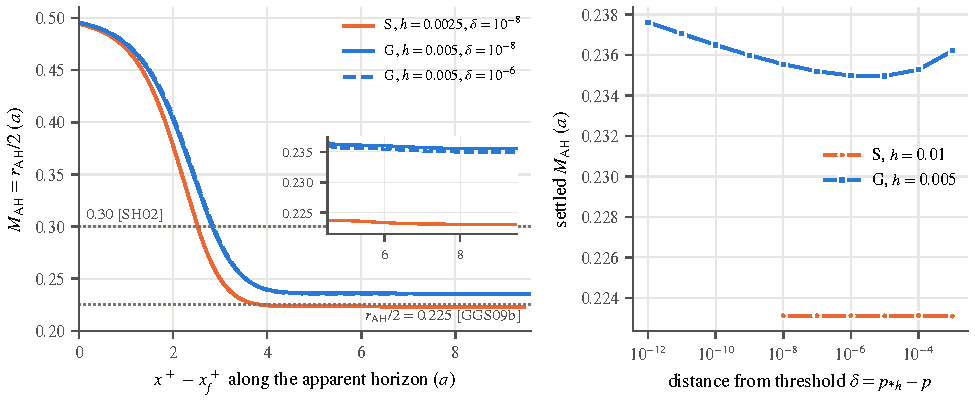
\includegraphics[width=\linewidth]{fig_mass.pdf}
\caption{Left: the Misner--Sharp mass on the apparent horizon against $x^+$ from the first trapped cell, for S and G;
the inset magnifies the plateau. The dotted lines are Shinkai and Hayward's $0.30a$~\cite{SH2002} and $r_\AH/2$ for the
radius $0.45a$ of Ref.~\cite{GGS2009b}. Right: the settled mass against the distance $\delta$ from threshold.}
\label{fig:mass}
\end{figure}

G settles higher, at $0.235548a$ ($r_\AH=0.4711a$) for $\delta=10^{-8}$, $1.25\times10^{-2}a$ above S at the same $h$
and $\delta$. The difference is the same at the three $h$, so it is not truncation error. Of it, $1.3\times10^{-3}a$ is
present at formation, and the rest is less negative-energy flux into the horizon afterwards; the normal field adds no
flux after formation. Unlike S, G's settled mass depends on $\delta$: over $10^{-12}\le\delta\le10^{-3}$ it has a minimum near
$\delta=10^{-5}$, and it rises by
$2\times10^{-4}$ to $6\times10^{-4}$ per decade as $\delta$ falls from $10^{-6}$ to $10^{-12}$, reaching $0.237622a$ at
$\delta=10^{-12}$. The rise per decade still grows at $10^{-12}$.

The published values compare as follows. All three earlier papers use a Misner--Sharp mass with $G=1$ in units of the
throat radius, so no unit factor separates them. Gonz\'alez, Guzm\'an and Sarbach's final radius $r_\AH=0.45a$ for a
vanishing perturbation~\cite{GGS2009b} agrees with $0.4462a$ to their two digits; their $m_\AH\approx0.22$ equals
$r_\AH/2$ if $m_\AH$ is the mass on the horizon, which their text implies but does not state. Shinkai and Torii's final
energy equals the static throat's own energy in each $D$, read shortly after the horizon forms: it is the formation
value, which is why it does not depend on the injected energy~\cite{ST2017}. Shinkai and Hayward's
$0.30a$~\cite{SH2002} is not reproduced. Run through the same chain, their own initial data give their injected energy
to within $3.8\%$ and their horizon coordinate to within $4.3\%$, but a settled mass of $0.22316a$ for their smallest
pulse against their $0.296a$. For their six runs this code's $M_\AH$ equals their printed values $1.5a$ to $2.5a$ of
$x^+$ after formation, while the mass is still falling (Fig.~\ref{fig:mass}).

\paragraph{Reading.} The black hole at the symmetric threshold has a finite mass, as type~I requires, and it is about a
quarter of the throat radius rather than half: the horizon forms at the throat, then swallows the ghost field's
negative energy and shrinks to $0.4462a$. The mass is not universal. A family that approaches a different static member
ends with a different mass, and for that family the mass keeps changing with the distance from threshold. In textbook
type~I collapse the mass scale comes from the field equations; here it comes from the throat, a property of the data,
and the static family has a direction (the asymmetry) along which the approached member can move.

\pending{\#266, \#267}{G's settled mass against the normal amplitude $B$ (with $B=0$ reproducing S's $0.2231a$), and
against the parameters $(\gamma_1, r_{\rm th})$ of the member at departure as $\delta\to0$. These will say whether the
settled mass is a function of the member the data leave.}

\pending{\#246}{The settled mass in $D=5$ and $6$, with $M=r^{n-1}/2$ on the horizon and a planted Tangherlini check per
$D$.}

\subsection{The expanding branch}\label{sec:expand}

Above threshold we follow the symmetric family to $t=283a$ in $D=4$ and $t=141a$ in $D=5$, for members tuned to
$\pst+10^{-6}$ and for larger amplitudes. By symmetry the line $x^+=x^-$ is the throat, a geodesic, and it stays the
minimum of $r$ on every slice to within one node. Let $\tau$ be its proper time and $H=\dd\ln r/\dd\tau$ its expansion
rate. An anti-trapped region contains the throat from the departure on, and no trapped cell forms.

$H$ does not settle. Over the last e-fold of $r$, $1/H$ is linear in $\tau$:
\begin{equation}
H=\frac{k}{\tau_s-\tau},\qquad k=2.0000\ (D=4),\qquad k=3.9875\ (D=5),\label{eq:ft}
\end{equation}
for the tuned members (Table~\ref{tab:expand}, Fig.~\ref{fig:expand}). So $r\propto(\tau_s-\tau)^{-k}$, and the areal
radius would diverge at the finite proper time $\tau_s$; the fitted exponents of $r$, $H$, the energy density $\rho$ and
the sectional curvature $K$ of the spheres are $-2.0000$, $-1.0000$, $-2.0000$ and $-2.0000$ in $D=4$. $\tau_s$ is an
extrapolation: the last cell is at $\tau_s-\tau=0.3151a$ in $D=4$ and $1.5874a$ in $D=5$. $H/W$ is $1.230$, $1.946$ and
$2.752$ at $r/a=10$, $25$, $50$ in $D=4$, far from a constant. The other members in $D=4$ have the same $k$ to
$4\times10^{-4}$; the amplitude mainly shifts $\tau_s$. The two resolutions agree on $H$ at fixed $r/a$ to
$5.0\times10^{-5}$ ($D=4$) and $4.1\times10^{-4}$ ($D=5$). The one-sided family G, read on its locus, gives
$k=1.9993$ to $1.9999$ for three members in $D=4$ and $k=3.9834$ for the tuned member in $D=5$.

\begin{table}[tbp]
\centering
\caption{The expanding throat of family S at the finer of two grid spacings ($h=0.01$ in $D=4$, $0.005/\sqrt2$ in
$D=5$): $k$ and $\tau_s$ from the linear fit of $1/H$ over the last e-fold of $r$, $|\rho|/H^2$ and $H/W$ at the radii
shown.}
\label{tab:expand}
\small
\begin{tabular}{rlllll}
\toprule
$D$ & member & $k$ & $\tau_s/a$ & $|\rho|/H^2$ at $r=50a$ & $H/W$ at $r/a=10$, $25$, $50$ \\
\midrule
4 & $\pst+10^{-6}$ & 2.0000 & 17.8902 & 4.0000 & 1.230, 1.946, 2.752 \\
4 & $p=0.01$ & 2.0000 & 10.0559 & 4.0000 & 1.232, 1.949, 2.756 \\
4 & $p=0.05$ & 2.0000 & 8.4334 & 3.9999 & 1.280, 2.024, 2.862 \\
4 & $p=0.2$ & 2.0004 & 6.1690 & 3.9985 & 1.769, 2.778, 3.924 \\
5 & $\pst+10^{-6}$ & 3.9875 & 15.0724 & 6.7525 & 0.847, 1.074, 1.279 \\
5 & $p=0.05$ & 3.9897 & 7.9180 & 6.7523 & 1.023, 1.297, 1.544 \\
\bottomrule
\end{tabular}
\end{table}

Two exact relations hold on the symmetric throat (Appendix~\ref{app:throat}). First, the field's gradient there is
purely radial, so in the throat's frame the radial pressure equals $\rho$ and the angular pressure equals $-\rho$; the
isotropic average gives
\begin{equation}
\bar w=\frac{p_\parallel+n\,p_\perp}{(n+1)\,\rho}=\frac{1-n}{1+n},\label{eq:wbar}
\end{equation}
$-1/3$ in $D=4$ and $-1/2$ in $D=5$, at every time (\emph{proved}). A de Sitter reading, $\bar w=-1$, is excluded on
this observer whatever the dynamics. Second, the Misner--Sharp mass and its flux law give
\begin{equation}
\frac{\dd H}{\dd\tau}=-\frac{n+1}{2}H^2-\frac{n-1}{2r^2}-\frac{\rho}{n},\label{eq:hdot}
\end{equation}
and with $H=k/(\tau_s-\tau)$ and $\rho=-cH^2$ it requires $c=n(1/k+(n+1)/2)$ once $r\to\infty$. That is $c=4$ for
$(n,k)=(2,2)$ and $27/4$ for $(3,4)$, against the measured $|\rho|/H^2=4.0000$ and $6.7525$. The data give $k$; this
relation does not.

Shinkai and Hayward's rate $1.1/a$ is the exponent of a fit $r/a=1+b_4e^{H(\tau-b_5)}$ to the early departure. The same
fit to our tuned member over $r/a\le r_{\max}$ gives $1.14$ to $1.16/a$ for $r_{\max}$ from $1.5$ to $10$: a window
average of a rate that keeps rising. Gonz\'alez, Guzm\'an and Sarbach's ``no apparent horizon'' on the expanding side
agrees with the absence of trapped cells; the marginal contours $r_+=0$ and $r_-=0$ bounding the anti-trapped region do
exist~\cite{GGS2009b}.

\begin{figure}[tbp]
\centering
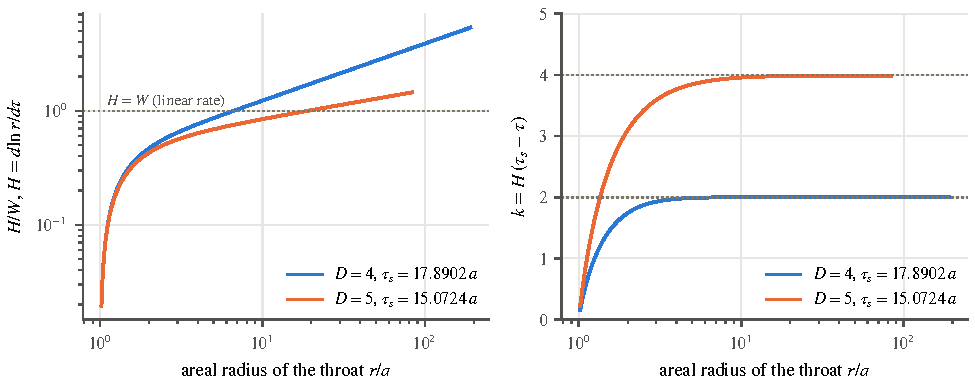
\includegraphics[width=\linewidth]{fig_expansion.pdf}
\caption{The throat of the symmetric family above threshold (members tuned to $\pst+10^{-6}$), against its areal radius.
Left: $H/W$; the throat leaves at the linear rate and then accelerates without a plateau. Right: $k=H(\tau_s-\tau)$ with
$\tau_s$ from the linear fit of $1/H$; it tends to $2$ in $D=4$ and to $3.99$ in $D=5$.}
\label{fig:expand}
\end{figure}

\paragraph{Reading.} The expanding throat is not a de Sitter phase. Its rate rises without bound on the fitted law, the
curvature rises with it ($K(\tau_s-\tau)^2\to4$ in $D=4$), and the symmetry fixes its equation of state at
$\bar w=(1-n)/(1+n)$. The ends of the grid gain mass, by exactly the ghost field's negative-energy flux through them. In
$D=4$ and $5$, $k=2$ and $k\approx4$, which fit $k=2(n-1)$; that is a \emph{conjecture} from two points.

\pending{\#230}{$k(n)$ from the scaling solution of the expanding throat: a closed form or a numerical scaling solution
whose $k$ and $c$ match Table~\ref{tab:expand} to $10^{-3}$, its prediction for $D=6$ tested by a run, and a longer
$D=4$ run that approaches $\tau_s$ more closely.}

\section{Consequences and limits}\label{sec:limits}

\begin{itemize}
\item \emph{The Ellis threshold follows the type~I lifetime law with the slope of the linear mode} in $D=4$, $5$ and $6$,
for families through the static wormhole. Those families start on the critical solution, so the test is of the
growth rate along its unstable direction in a nonlinear code, not of the approach of generic data.
\item \emph{Generic data in $D=4$ approach an asymmetric member} and leave at its rate. Which member a given family selects
is not predicted here. In $D=5$ the member drifts during the stall, and the lifetime is not one logarithm (\#255
pending). G in $D=6$ was not read on the locus.
\item \emph{The threshold mass is finite and non-universal.} It is $0.2231a$ for S, the value of Ref.~\cite{GGS2009b},
and $0.2355a$ for G at $\delta=10^{-8}$, still changing with $\delta$ at $10^{-12}$. Whether it is a function of the
member at departure is open (\#266, \#267). Masses were measured in $D=4$ only (\#246).
\item \emph{``Settled'' means to $e^{-f}=1.57\times10^6$ on the apparent horizon}, $9.4a$ of $x^+$ after formation, not
to the event horizon or to null infinity; the horizon flux had returned once before it died, so a later change is not
excluded by the data.
\item \emph{Shinkai and Hayward's $0.30a$ remains unexplained.} Their reading two time units after formation would give
it, and their uniform grid may not resolve the horizon at the times they read; that is a \emph{conjecture}. A uniform
grid of their size run with this code's kernel loses the horizon before their reading time and reads high, by less
than the difference.
\item \emph{The expanding throat diverges in finite proper time on the fitted law}, with $k=2.0000$ and $3.99$; whether
it reaches $\tau_s$ is not measured, the observer is the symmetric throat only, and $k=2(n-1)$ is a \emph{conjecture}
(\#230 pending).
\item \emph{The roundoff floor}: $\pst$ is determined to about $10^{-12}$ by roundoff (\#227 pending).
\item \emph{Not studied}: the second collapse window on the expanding side~\cite{GGS2009b}, non-spherical
perturbations, and wormholes of a ghost with a potential or a charge.
\end{itemize}

\section{Computations}\label{sec:computations}

\paragraph{The code and its checks.} The evolution is \texttt{dn.py}, with a numba kernel for production and a numpy
kernel as reference; on three grids, one with excision, the two are bit-identical. The field equations were checked
symbolically against a brute-force Ricci tensor of the full metric for $D=4$--$7$ (\texttt{derive.py}, 25 checks). Its
checks (\texttt{checks.py}, 11 of 11 pass) run exact solutions through the code:
\begin{itemize}
\item the static wormhole stays static to the truncation error, with observed orders $2.045$, $1.978$ ($D=4$) and
$2.059$, $2.002$ ($D=5$);
\item the Tangherlini black hole~\cite{Tangherlini1963} in Kruskal coordinates, $D=4$, $5$, $6$, with its horizon
position at orders $1.999$ to $2.000$;
\item an exact dynamical ghost solution of the self-similar Roberts family~\cite{Roberts1989,Maeda2009} in $D=4$, which
crosses $r_+=0$ and $r_-=0$, with its horizon lines at slopes $0.666668$ and $1.499991$ against $2/3$ and $3/2$ and no
misclassified cell;
\item the growth rate of the tuned static wormhole, $1.181988$ and $1.181934$ at $h=0.02$, $0.01$ against $W=1.181970$
in $D=4$.
\end{itemize}
Each of 14 mutations (a sign, a coefficient, a dropped corrector) fires exactly its declared checks.

\paragraph{The threshold runs.} A planted type~I series with known slope and $p_*$, through the same bisection and fit
code, recovers $p_*$ and has $1/W$ inside the fit spread for 40 of 40 noise seeds in each $D$; a series planted with
the slope $1/(\sqrt2W)$, the null-coordinate time unit, is rejected in 40 of 40. In $D=6$ the growth rate was checked
before any bisection, $2.160530$ and $2.162551$ against $W=2.164860$. The criteria and the mutations were written down
before the runs of record, in the raw-output repository.

\paragraph{The second code.} The reviewer wrote \texttt{threshold\_check.py} for family S. It integrates the
background and the ray constraint itself, uses its own diamond scheme on the half $x^+\ge x^-$, and places its events at
$r=a/2$ and $2a$ on the throat, interpolated in $t$. It shares no code with \texttt{dn.py}; it shares the field
equations, the family's definition and $W$. Its $\pst$ agrees with the first code's to a relative $1.9\times10^{-4}$, so
the two schemes' truncation seeds are close, and its slopes are those of Table~\ref{tab:life}. Its mutations (a wrong
oracle slope, a shifted $\pst$ in the fit, the $\sqrt2$ time unit) fire exactly their targets; the time-unit mutation
gives $0.598243$ against $1/(\sqrt2W)=0.598244$.

\paragraph{The review checks.} Each result was reviewed on another machine with a check that shares no code with the
code under test except as stated.
\begin{itemize}
\item \emph{ind39} derives the equations from its own Ricci tensor (sympy residual 0) and runs the tuned growth rate in
$D=6$: $2.160443$ and $2.162520$ against $2.164860$.
\item \emph{ind40} is the second code above.
\item \emph{ind41}, a half-domain march on a uniform grid, gives $M_\AH=0.30315a$ at $e^{-f}=4.074$ on the horizon, and
agrees with the chain to $1.2\times10^{-4}$ up to $e^{-f}=11.96$. A uniform grid cannot reach the plateau, so the
settled value rests on the chain, its planted Schwarzschild horizon (mass error $1.684\times10^{-6}$ at $h=0.0025$,
second order) and its convergence at four $h$.
\item \emph{ind213}, the second code run without stopping, gives $k=2.00001$ to $2.00040$ for the eight $D=4$ runs.
\item \emph{ind225} interpolates $T(\gamma_1)$ from three published values and gives the e-fold $0.847466a$ at the
stall member, against the measured $0.8475a$.
\item \emph{ind226} is below.
\end{itemize}
G's settled mass has no independent code: the second code is the symmetric half domain. It rests on the chain's
planted cases, unchanged, and on its convergence at three $h$; a rerun on another machine gave the plateau to
$8.05\times10^{-7}$.

\paragraph{The constraint plateau.} The constraint maximum along the bracketing runs falls by four per halving of $h$,
except at the finest $h$ in $D=5$ and $6$, where it stops falling. That is roundoff. The second difference of $r$ in
$C_{\pm\pm}$ carries the roundoff of each node as $\epsilon/h^2$, and $r^{n-1}C_{++}$ is constant along $x^-$
(Appendix~\ref{app:equations}), so a violation made where $r$ is large is amplified on its way to the throat. On a
fixed slab of the static wormhole in $D=6$ the ratios per halving are $4.204$, $3.758$ and $1.337$; in binary128
arithmetic the same slabs fall by $4.0$ to $4.2$ at every halving of every set; and added relative noise
$256\cdot2^{-52}$ per node raises the finest-$h$ maximum by a factor $113$ ($D=6$) and $57$ ($D=5$). The reviewer's own march gives $4.197$,
$3.833$ and $1.356$. The roundoff error of $r$ itself is $1.4\times10^{-11}$ against a truncation error of
$4.1\times10^{-4}$ ($D=6$, $h=0.00125$), so the plateau does not bear on $\pst$ or on the slopes.

\paragraph{Numbers and figures.} Every number in this paper is read from the output files in
\path{notes/wormhole_evolution/} (and, for the checks of the code and the reviews, from the raw-output repository) by
\path{paper/5-ellis-threshold/paper_numbers.py}, which checks that this text prints it and exits non-zero otherwise; a
mutation of a source number makes it fail. The figures are drawn by \path{paper/5-ellis-threshold/make_figures.py} from
the runs of record.

\section*{How this work was done}

Nathan Moinvaziri posed the problem and directed the work. Claude (Anthropic), run as agents on several machines,
drafted the evolution code, the analysis scripts and this text. A separate reviewing Claude session checked each result
on another machine with code it wrote independently: the second double-null code \texttt{threshold\_check.py} and the
review checks ind39, ind41, ind213, ind225 and ind226 of Sec.~\ref{sec:computations}.

\paragraph{Reproducibility.} The repository is \url{https://github.com/nmoinvaz/negative-mass}: the code and notes are in
\path{notes/wormhole_evolution/}, and the raw output, with the criteria written before each run of record, is in
\url{https://github.com/nmoinvaz/negative-mass-raw} (folders \texttt{I39}, \texttt{I40}, \texttt{I41}, \texttt{I213},
\texttt{I225}, \texttt{I226}, \texttt{I253}).

\appendix

\section{The equations}\label{app:equations}

With the metric $-2e^{-f}\dd x^+\dd x^-+r^2\dd\Omega_n^2$ and $R_{ab}=\sum_k\varepsilon_k\partial_a\phi_k\partial_b\phi_k$,
the Ricci tensor gives Eqs.~\eqref{eq:evol}--\eqref{eq:constraints} (\emph{checked symbolically}: the brute-force
Ricci tensor of the full metric for $D=4$--$7$ against the reduced expressions with $n$ symbolic). Three identities
follow (\emph{checked symbolically}):
\begin{itemize}
\item \emph{Constraint propagation.} $\partial_-C_{++}=-(n-1)(r_-/r)\,C_{++}$, so $r^{n-1}C_{++}$ is constant along
$x^-$, and likewise $r^{n-1}C_{--}$ along $x^+$.
\item \emph{Mass flux.} With the constraints satisfied, $\partial_+M=-(r^n/n)\,e^fr_-\sum_k\varepsilon_k\phi_{k+}^2$ and
$\partial_-M=-(r^n/n)\,e^fr_+\sum_k\varepsilon_k\phi_{k-}^2$ for the mass~\eqref{eq:ms}.
\item \emph{Stress.} $T_{+-}=0$, $T_{\pm\pm}=\sum_k\varepsilon_k\phi_{k\pm}^2$, and the angular pressure is
$e^f\sum_k\varepsilon_k\phi_{k+}\phi_{k-}$.
\end{itemize}

\section{The symmetric throat}\label{app:throat}

Let the data be mirror symmetric: $\phi(x^+,x^-)=-\phi(x^-,x^+)$ for the ghost field $\phi$ ($\varepsilon=-1$), and $r$,
$f$ symmetric. The evolution preserves this. On the throat $x^+=x^-$ then $\phi=0$, $r_+=r_-$ and $\phi_+=-\phi_-$. The
unit normal to the slices there is $u=e^{f/2}(\partial_++\partial_-)/\sqrt2$, and with $T_{ab}=\varepsilon(\partial_a
\phi\partial_b\phi-\tfrac12g_{ab}(\partial\phi)^2)$ and $g_{+-}=-e^{-f}$:
\begin{itemize}
\item $T_{+-}=\varepsilon(\phi_+\phi_--\phi_+\phi_-)=0$, so $\rho=T_{uu}=\tfrac12e^f(T_{++}+T_{--})=\varepsilon e^f\phi_+^2$;
\item the radial pressure is $p_\parallel=T_{ll}=\tfrac12e^f(T_{++}+T_{--})=\rho$;
\item the angular pressure is $p_\perp=\varepsilon e^f\phi_+\phi_-=-\varepsilon e^f\phi_+^2=-\rho$.
\end{itemize}
Hence $\bar w=(p_\parallel+np_\perp)/((n+1)\rho)=(1-n)/(1+n)$ wherever $\rho\ne0$, which is Eq.~\eqref{eq:wbar}
(\emph{proved}). A homogeneous ghost field, $\phi_+=\phi_-$, would instead have $\bar w=+1$; the code recovers this on an
exact open Friedmann solution with a homogeneous ghost (\texttt{expansion.py}, control W1).

\emph{The rate equation.} On the throat $r_l=0$, so $(\nabla r)^2=-\dot r^2$ with $\dot r=\dd r/\dd\tau$, and the mass
is $m=\tfrac12r^{n-1}(1+\dot r^2)$. Along the throat $\dd/\dd\tau=e^{f/2}(\partial_++\partial_-)/\sqrt2$ and
$\dot r=\sqrt2e^{f/2}r_+$. The flux laws of Appendix~\ref{app:equations}, with $r_+=r_-$ and $\phi_+^2=\phi_-^2$, give
\begin{equation}
\dot m=-\frac{e^{f/2}}{\sqrt2}\,\frac{r^n}{n}\,e^f\,2r_+\,\varepsilon\phi_+^2=-\frac{r^n}{n}\,\rho\,\dot r.
\end{equation}
Differentiating $m$ and dividing by $r^{n-1}\dot r$ gives $\ddot r/r=-(n-1)(1+\dot r^2)/(2r^2)-\rho/n$, and with
$H=\dot r/r$, $\dot H=\ddot r/r-H^2$, this is Eq.~\eqref{eq:hdot} (\emph{proved}, given the flux laws). If
$H=k/(\tau_s-\tau)$ then $\dot H=H^2/k$ and $r\propto(\tau_s-\tau)^{-k}$, so $1/r^2=o(H^2)$ for $k>1$, and
$\rho=-cH^2$ requires $c=n\,(1/k+(n+1)/2)$.

\begin{thebibliography}{99}

\bibitem{Ellis1973} H. G. Ellis, ``Ether flow through a drainhole: a particle model in general relativity,'' J. Math.
Phys. \textbf{14}, 104 (1973), doi:10.1063/1.1666161.
\bibitem{Bronnikov1973} K. A. Bronnikov, ``Scalar-tensor theory and scalar charge,'' Acta Phys. Pol. B \textbf{4}, 251
(1973).
\bibitem{GGS2009a} J. A. Gonz\'alez, F. S. Guzm\'an and O. Sarbach, ``Instability of wormholes supported by a ghost scalar
field. I. Linear stability analysis,'' Class. Quantum Grav. \textbf{26}, 015010 (2009), arXiv:0806.0608.
\bibitem{GGS2009b} J. A. Gonz\'alez, F. S. Guzm\'an and O. Sarbach, ``Instability of wormholes supported by a ghost scalar
field. II. Nonlinear evolution,'' Class. Quantum Grav. \textbf{26}, 015011 (2009), arXiv:0806.1370.
\bibitem{TS2013} T. Torii and H. Shinkai, ``Wormholes in higher dimensional space-time: exact solutions and their
linear stability analysis,'' Phys. Rev. D \textbf{88}, 064027 (2013), arXiv:1309.2058.
\bibitem{P3} N. Moinvaziri, ``The instability of ghost-scalar wormholes at large dimension'' (2026), in preparation;
\path{paper/3-wormhole-largeD} in the accompanying repository.
\bibitem{SH2002} H. Shinkai and S. A. Hayward, ``Fate of the first traversible wormhole: black-hole collapse or
inflationary expansion,'' Phys. Rev. D \textbf{66}, 044005 (2002), arXiv:gr-qc/0205041.
\bibitem{ST2017} H. Shinkai and T. Torii, ``Nonlinear dynamics in the Einstein--Gauss--Bonnet gravity,'' Phys. Rev. D
\textbf{96}, 044009 (2017), arXiv:1706.02070.
\bibitem{XCY2025} A. Xu, X. Y. Chew and D. Yeom, ``Dynamics of Bronnikov--Ellis wormhole with double-null simulation,''
JCAP \textbf{08} (2025) 012, arXiv:2503.07610.
\bibitem{Kain2026} B. Kain, ``Dynamical wormholes,'' Class. Quantum Grav. \textbf{43}, 045014 (2026), arXiv:2602.18231.
\bibitem{SN2026} N. M. Shirokov and I. Nachevsky, ``Binary Ellis--Bronnikov wormholes in 3+1 numerical relativity:
mergers, fly-bys and gravitational waves,'' arXiv:2610.13206 (2026).
\bibitem{CCB1996} M. W. Choptuik, T. Chmaj and P. Bizo\'n, ``Critical behavior in gravitational collapse of a
Yang--Mills field,'' Phys. Rev. Lett. \textbf{77}, 424 (1996), arXiv:gr-qc/9603051.
\bibitem{GMG2007} C. Gundlach and J. M. Mart\'in-Garc\'ia, ``Critical phenomena in gravitational collapse,'' Living Rev.
Relativ. \textbf{10}, 5 (2007), arXiv:0711.4620.
\bibitem{GHMG2025} C. Gundlach, D. Hilditch and J. M. Mart\'in-Garc\'ia, ``Critical phenomena in gravitational
collapse,'' arXiv:2507.07636 (2025).
\bibitem{MisnerSharp1964} C. W. Misner and D. H. Sharp, ``Relativistic equations for adiabatic, spherically symmetric
gravitational collapse,'' Phys. Rev. \textbf{136}, B571 (1964), doi:10.1103/PhysRev.136.B571.
\bibitem{Tangherlini1963} F. R. Tangherlini, ``Schwarzschild field in $n$ dimensions and the dimensionality of space
problem,'' Nuovo Cimento \textbf{27}, 636 (1963), doi:10.1007/BF02784569.
\bibitem{Roberts1989} M. D. Roberts, ``Scalar field counterexamples to the cosmic censorship hypothesis,'' Gen. Relativ.
Gravit. \textbf{21}, 907 (1989), doi:10.1007/BF00769864.
\bibitem{Maeda2009} H. Maeda, ``Simple analytic model of wormhole formation,'' Phys. Rev. D \textbf{79}, 024030 (2009),
arXiv:0811.2962.

\end{thebibliography}

\end{document}
